%\documentclass[12pt,aspectratio=169]{beamer}
\documentclass[12pt]{beamer}
%\documentclass[20pt,handout]{beamer}
\usetheme{Dresden}
\usepackage{graphicx}
\usepackage[ngerman]{babel}
\usepackage[T1]{fontenc}
\usepackage[utf8]{inputenc}
\usepackage{tikz}
\setbeamertemplate{footline}[frame number]

\newcommand{\cc}[1]{\includegraphics[height=2cm]{img/#1.pdf}}
\usepackage{ifthen}
\newcommand{\license}[2][]{\\#2\ifthenelse{\equal{#1}{}}{}{\\\scriptsize\url{#1}}}
\usepackage{textcomp}

\pgfdeclareimage[height=0.8cm]{c3d2logo}{./img/c3d2Skull-v4.pdf} 


\pgfdeclarelayer{foreground}
\pgfsetlayers{main,foreground}
\logo{\pgfputat{\pgfxy(-1,0)}{\pgfbox[center,base]{\pgfuseimage{c3d2logo}}}}

\title{BuFaK WiSo\\Informationssicherheit \& Datenschutz}
\author{\small \texttt{vv01f} \\ \Large Chaos Computer Club Dresden \\ \texttt{www.c3d2.de}  }
\date{01.05.2015 ab 09:30 Uhr, HTW Dresden S\,308a }

\begin{document}
\maketitle

\section{Einleitung}
\subsection{}

\begin{frame}
	\frametitle{Wer steht hier vorn und wie wichtig ist das?}
		\begin{center}
			
\includegraphics[height=0.5\textheight]{./img/fingerabdruck.pdf} \\
			\texttt{7247 DD6D CB19 A11D 4BCE  9536 24CB A706 AD26 D9FB}
		\end{center}
\end{frame}

\begin{frame}
	\frametitle{Wer steht hier vorn}
	\begin{itemize}
		\item Chaos Computer Club Dresden (\url{https://c3d2.de/})
			\note{GCHQ am Pirnaischen Platz, Lingerstraße 3, 01069 Dresden https://c3d2.de/space.html}
		\item Chaos macht Schule
		\item Datenspuren: 24. -- 25. Oktober 2015 \url{https://datenspuren.de/}
		\item StuRa der HTW Dresden \url{http://stura.htw-dresden.de/}
		\item Freie Software \& Freies Wissen \url{https://fsfw-dresden.de/}
	\end{itemize}
\end{frame}

\begin{frame}
	\frametitle{Was das hier wird}
	\begin{itemize}
		\item Kurze Einführung in das Themengebiet
		\item Beispiele aus der Praxis
		\item Erfahrungsaustausch
	\end{itemize}
\end{frame}

\section{ITSec \& DSch}
\subsection{Informationssicherheit}

\begin{frame}
	\frametitle{Was ist Information?}
	\begin{itemize}
		\item jedes Datum
		\item atomare Eigenschaft
		\item Relation von Informationen
		\item Inhalt einer Antwort
	\end{itemize}
\end{frame}

\begin{frame}
	\frametitle{Und was sind dann Daten?}

\begin{columns}[T]
    \begin{column}{.3\textwidth}
    \begin{block}{BCD ASCII}
		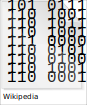
\includegraphics[width=1.9cm]{./img/WikipediaBinary.pdf}
    \end{block}
    \end{column}
    \begin{column}{.7\textwidth}
     \begin{block}{abstrahiert}
	\begin{itemize}
		\item Nicht-eindeutige Definition
		\item Abgrenzung von Information
		\item Formulierte Angaben
		\item Einsatz v. Sprache, Kodierung/Alphabet
		\item Primärziel: Maschinentauglichkeit
	\end{itemize}
    \end{block}
    \end{column}
  \end{columns}

\end{frame}

\begin{frame}
	\frametitle{Informationssicherheit, Aspekte der}
	\begin{itemize}
		\item Verfügbarkeit
		\item Integrität
		\item Vertraulichkeit
		\item weitere Ausprägungen davon: Authentizität, (Nicht-)Abstreitbarkeit, Zurechenbarkeit
		\item für \textbf{IT-Systeme}
	\end{itemize}
\end{frame}

\begin{frame}
	\frametitle{Informationssicherheit, Gefährungen nach Häufigkeit}
	\begin{itemize}
		\item Personell (z.B. Unkenntnis, Sabotage)
		\item Immateriell (fehlende Rechte, Software)
		\item Materiell (Ermüdung, Unzulänglichkeit)
	\end{itemize}
\end{frame}

\begin{frame}
	\frametitle{Informationssicherheit, Maßnahmen geg. Gefährdungen (n:1)}
	\begin{itemize}
		\item Technisch, vorausschauend, u.a. Automatisierung
		\item Organisatorisch, ersparen von Automatisierung
		\item Operativ, kurzfristige Eingriff im Notfall
	\end{itemize}
\end{frame}

%\section{}
\subsection{Datenschutz}

\begin{frame}
	\frametitle{Unterschied zur Informationssicherheit}
	\begin{itemize}
		\item Nicht mehr nur in IT-Systemen
		\item Personenbezogene Daten (§3\,Abs.\,1 BDSG)
		\item weitere schutzbedürftige Informationen, z.B. zu Organisationen
		\item auch Schutz von Geheimnissen: Verschlusssachen, Informationsvorbehalt
	\end{itemize}
\end{frame}

\begin{frame}
	\frametitle{Prozesse}
	\begin{itemize}
		\item Erhebung (Beschaffung)
		\item Verarbeitung (Speichern, Verändern, Übermitteln, Sperren, Löschen)
		\item Nutzung (Verwendung ohne Verarbeitung)
	\end{itemize}
\end{frame}

\begin{frame}
	\frametitle{Datenvermeidung und -sparsamkeit}
	\begin{quotation}
		Die \${Prozesse} pers.Dat. \emph{und die Auswahl und Gestaltung} [der Systeme] sind an dem Ziel auszurichten, so wenig pers.Dat. wie möglich zu \${prozessieren}. Insbesondere [\ldots] anonymisieren oder zu pseudonymisieren, soweit dies [\ldots] möglich ist und keinen [\ldots] unverhältnismäßigen Aufwand erfordert.
	\end{quotation}
\end{frame}

\section{Praxis}
\subsection{}

\begin{frame}
	\frametitle{Umgangsformen}
	\begin{itemize}
		\item Wem sollte man was preisgeben/posten (und was eher nicht)?
		\item Geburtstagsglückwünsche bei feierlicher Imma
		\item redundante, unnötige Adressierung bei Email
		\item unnötger Geschlechtsbezug
		\item nicht sachgerechte Identifikationspflichten
	\end{itemize}
\end{frame}

\begin{frame}
	\frametitle{Einzelfall: Unbefugte Weitergabe von pers.Dat.}
	\begin{itemize}
		\item Telefonnummer - weil es schnell gehen muss
		\item Namen in Bezug auf Problemfälle
		\item Geburtsdatum
		\item Fotos
	\end{itemize}
\end{frame}

\begin{frame}
	\frametitle{Massenhafte Weitergabe: FSR-Wahlbenachrichtigung 2014}
	\begin{itemize}
		\item Ungesicherte Nachrichtenübermittlung
		\item Unnötig viele Informationen in Email
		\begin{itemize}
			\item Name, Vorname, s-Nummer
			\item Postalische Anschrift
			\item Geburtsdatum
			\item Studiengang
		\end{itemize}
		\item Ohne Zurechenbarkeit
		\item Unberechtigte Weitergabe
	\end{itemize}
\end{frame}

\begin{frame}
	\frametitle{Unverhältnismäßigkeiten}
	\begin{itemize}
		\item Matrikel und Name auf Prüfungen
		\item Unterschriften für Teilnahme/Abgabe von Prüfungen
		\item Statistik Anwesenheit ohne Anwesenheitspflicht
	\end{itemize}
\end{frame}

\begin{frame}
	\frametitle{Verweigerung von Schutzmaßnahmen}
	\begin{itemize}
		\item Verweigerung von Verbindlichkeit
		\item Verunmöglichung der Vertraulichkeit
		\item Vorlagen-Texte in Emails
	\end{itemize}
\end{frame}

\subsection{}

\begin{frame}
	\frametitle{Beratung von Studenten}
	\begin{itemize}
		\item Weiterleiten von Email an private Adresse
		\item Nutzung unsicherer Authentifizierungsmethoden
		\item Empfehlung von proprietären SaaS-Anbietern
		\item HRZ: Fehlende, veraltete oder falsche Informationen und Anleitungen
	\end{itemize}
\end{frame}

\begin{frame}
	\frametitle{Tracking}
	\begin{itemize}
		\item Anwesenheitslisten
		\item Cookies, Like Buttons, Werbe- und Statistiknetzwerke
		\item "`Soziale"' Netzwerke
	\end{itemize}
\end{frame}

\begin{frame}
	\frametitle{Passwörter}
	\begin{itemize}
		\item schlechter Standard: Geburtsdatum o.ä.
		\item Keine einfachen Wörter
		\item Groß-, Kleinbuchstaben, Ziffern, Sonderzeichen
		\item Verschiedene Passwörter nutzen!
		\item Mehrfaktorauthentifizierung 
	\end{itemize}
\end{frame}

\begin{frame}
	\frametitle{Orga BuFaK}
	\begin{itemize}
		\item Einbinden von ungeprüften Drittdiensten
		\item Datenerhebung mit Google docs
	\end{itemize}
\end{frame}

\begin{frame}
	\frametitle{Diskussion}
	\begin{itemize}
		\item Der Zugang [zu Informationen] sollte unbegrenzt und vollständig sein.
		\item Alle Informationen müssen frei sein.
		\item Mißtraue Autoritäten – fördere Dezentralisierung.
		\item Beurteile [\ldots] nach [Taten], und nicht nach [personenbezogenen Kriterien].
		\item \,[Wir können unser] Leben zum Besseren verändern.
		\item Mülle nicht in den Daten anderer Leute.
		\item Öffentliche Daten nützen, private Daten schützen.
		\note{ Hackerethik \url{http://www.ccc.de/de/hackerethik}, Hackers von S.\,Levy \url{http://c3jemx2ube5v5zpg.onion/?document=view&id=374} }
	\end{itemize}
\end{frame}

\begin{frame}
	\frametitle{Copyleft}
	\begin{center}
		\cc{cc-by-sa-License} \\
		\footnotesize\url{https://creativecommons.org/licenses/by-sa/3.0/}
	\end{center}
\end{frame}

\end{document}
